% General Paper Template created by Adam Green
% Last revised 3/2/18

\documentclass[12pt]{article}

%%%%%%%%%%%%%%%%%%%%%%%%%%%%
% Standard Packages
%%%%%%%%%%%%%%%%%%%%%%%%%%%%
\usepackage{amsmath,amsfonts,amsthm,amssymb}
\usepackage[margin = 2cm]{geometry}


%%%%%%%%%%%%%%%%%%%%%%%%%%%%
% Graphical Packages
%%%%%%%%%%%%%%%%%%%%%%%%%%%%
\usepackage{graphicx}
\usepackage{subfig}
\usepackage{float}
\usepackage{tikz}
\usepackage{wrapfig}
% Syntax: \begin{wrapfig}[lineheight]{position}{width}

%\usepackage{tikz-3dplot}
%\usepackage{pgfplots}

\graphicspath{{Figures/}} % set directory for figures

%%%%%%%%%%%%%%%%%%%%%%%%%%%%
% Colors
%%%%%%%%%%%%%%%%%%%%%%%%%%%%
\usepackage{xcolor}

\definecolor{myblue1}{RGB}{76, 142, 185}
\definecolor{myblue2}{RGB}{25, 100, 126}
\definecolor{myblue3}{RGB}{41, 110, 180}

\definecolor{mygreen1}{RGB}{88,165,87}
\definecolor{mygreen2}{RGB}{91,165,98}

\definecolor{myred1}{RGB}{221, 28, 26}
\definecolor{mypurple}{RGB}{122,48,108}


%%%%%%%%%%%%%%%%%%%%%%%%%%%%
% Table and Array Packages
%%%%%%%%%%%%%%%%%%%%%%%%%%%%
\usepackage{tabu}
\usepackage{booktabs}


%%%%%%%%%%%%%%%%%%%%%%%%%%%%
% Citation Packages
%%%%%%%%%%%%%%%%%%%%%%%%%%%%
\usepackage{hyperref}
\hypersetup{allcolors = myblue1,
	allbordercolors = myblue1, 
	filecolor = myblue1, 
	linkbordercolor = myblue1,
	urlbordercolor = white
}

\usepackage{cleveref}
\crefname{equation}{Eqn.}{Eqns.}
\crefname{figure}{Fig.}{Figs.}
\crefname{table}{Tab.}{Tabs.}

%\usepackage{caption}
%	\captionsetup{format = , justification= }

%%%%%%%%%%%%%%%%%%%%%%%%%%%%
% Text Formatting packages
%%%%%%%%%%%%%%%%%%%%%%%%%%%%
\usepackage{multicol}
\usepackage{parskip} 
\usepackage{indentfirst} 
\setlength{\parindent}{0.75cm}
\usepackage{fancyhdr}
%	\pagestyle{fancy}
\usepackage{enumerate}
\usepackage{wrapfig}
\usepackage{lipsum}
\usepackage{xhfill}


%%%%%%%%%%%%%%%%%%%%%%%%%%%%
% Custom Commands
%%%%%%%%%%%%%%%%%%%%%%%%%%%%
% Red marks to get attention
\newcommand{\red}[1]{\textbf{\textcolor{myred1}{#1}}} % Red Text
\newcommand{\redmark}{\textcolor{myred1}{\rule{4mm}{4mm} }} % Red Dash
\newcommand{\redline}{\noindent\xhrulefill{myred1}{3pt}} % Red Rule


% Lowercase Captial Letters
\newcommand{\scap}[1]{\textsc{\MakeLowercase{#1}}} % Makes caps small so it doesnt SHOUT


% Math Commands: first and second order partials, Laplacian
\newcommand{\evaluate}{\Bigr\rvert}
\newcommand{\ppd}[1]{\frac{\partial}{\partial#1}}
\newcommand{\ppsd}[1]{\frac{\partial^2}{\partial #1^2}}
\newcommand{\ppnd}[2]{\frac{\partial #1}{\partial #2}}
\newcommand{\ppsnd}[2]{\frac{\partial^2 #1}{\partial #2^2}}
\newcommand{\lap}{\nabla^2}

% Quantum bra- ket- commands
\newcommand{\bra}[1]{\langle #1 |}
\newcommand{\ket}[1]{| #1 \rangle}
\newcommand{\bracket}[2]{\langle #1 | #2 \rangle}

% Redfine equation and figure references to include "Eqn. ()" and "Fig. _"
%\newcommand{\figref}[1]{Fig.\ \ref{#1}}
%\let\originaleqref=\eqref
%\renewcommand{\eqref}{Eqn.\ \originaleqref}


% Custom Matrix Spacing
% Syntax: \begin{matrix}[scale]
\makeatletter
\renewcommand*\env@matrix[1][\arraystretch]{%
	\edef\arraystretch{#1}%
	\hskip -\arraycolsep
	\let\@ifnextchar\new@ifnextchar
	\array{*\c@MaxMatrixCols c}}
\makeatother


% Email Commands: Taken from Flip
% Syntax: \email{email}
\newcommand{\email}[1]{\href{mailto:#1}{\textcolor{mygreen1}{#1}}}

% Institution Environment: Taken From Flip
\newenvironment{institutions}[1][2em]{\begin{list}{}{\setlength\leftmargin{#1}\setlength\rightmargin{#1}}\item[]}{\end{list}}

% Link to External Webpage
% Syntax: \link{url}
\newcommand{\link}[1]{\href{#1}{\textcolor{mygreen1}{\texttt{#1}}}}


%%%%%%%%%%%%%%%%%%%%%%%%%%%%
% Document Specific Commands
%%%%%%%%%%%%%%%%%%%%%%%%%%%%








\begin{document}
	\begin{center}
		
		{\LARGE \bf Noise Fundamentals}\\
		
		\vspace{0.5cm}
		
		\textbf{Adam Green}, \textbf{Guillermo Acuna}\\
		
		\texttt{\footnotesize \email{agree019@ucr.edu}},
		\texttt{\footnotesize \email{gacun002@ucr.edu}}
		
		\vspace{0.5cm}
		
		
		\begin{institutions}[2.25cm]
			\footnotesize
			{\it 
				Department of Physics \& Astronomy, 
				University of  California, Riverside, 
				CA 92521	    
			}    
		\end{institutions}
		
		\vspace{0.5cm}
	\end{center}

	\vspace{0.5cm}
	
	\begin{abstract}
		In this experiment we utilize Johnson and shot noise to measure Boltzmann's constant and the fundamental electric charge. For Johnson noise, we find that the data obeys Nyquist's theorem and we measure the power spectral density against resistance and temperature. From these measurements we extract Boltzmann's constant to be \red{kb}. For shot noise, we measure the power spectral density against bandwidth and photodiode current. Similarly, we find that the data obeys the linear relationship predicted by Schottky's theorem. From this, we extract the fundamental electric charge to be \red{e}.
	\end{abstract}
	
	\tableofcontents

	\pagebreak

	\section{Introduction}
	
	\subsection{Nyquist's Theorem}
	\begin{wrapfigure}{r}{0.4\textwidth}
		\includegraphics[width=0.4\textwidth]{circuit1.png}
		\caption{Idealized circuit for deriving Johnson Noise}
		\label{circuit1}
	\end{wrapfigure}
	For any electrical conductor at nonzero absolute temperature, the electrons inside it are thermally excited and randomly fluctuating. This random excitement creates a fluctuating voltage across the conductor. Since the motion is random, the average of this voltage is zero, but the size of the fluctuations can be quantified by time-averaging the square of the voltage. 
		
	For an impedance matched circuit like that shown in \cref{circuit1}, the energy traveling along the lossless line $L$ is perfectly absorbed without reflection. Applying boundary conditions, the voltage on either end of the transmission line must be equivalent. This occurs when the propagating electromagnetic wave has a wavelength $\lambda$ which satisfies $L=n\lambda$ where $n$ is an integer. The frequency of this propagation mode is $f = nc/L$, where $c$ is the speed of light.
	
	If we assume that the system is at some nonzero temperature $T$, then the average energy for each propagation mode $f$ obeys the Planck distribution:
	\begin{equation}
		\epsilon (f) = \frac{hf}{e^{(hf/k_BT)}-1}
	\end{equation}
	where $h$ is Planck's constant, $k_B$ is Boltzmann's constant, and $T$ is the temperature of the system. For frequencies in the range $f$ to $f+\Delta f$, the average power incident on the source resistor $R_s$ is:
	\begin{equation}
		P_i = \Delta f \frac{hf}{e^{(hf/k_BT)}-1}
	\end{equation}
	
	Since the electrons in the conductor are thermally excited, we treat them as a randomly fluctuating voltage source $V_J$. This generates a current $I_J$ in the transmission line. If the source and load resistor are equivalent, the average power emitted by the source resistor is:
	\begin{equation}
		P_e = R_s \langle I_J^2 \rangle = \frac{\langle V_J^2\rangle}{4R}
	\end{equation}
	
	Finally, since all components of the circuit are assumed to be ideal and the transmission line is lossless, the power incident must equal the power emitted by the source resistor, $P_i = P_e$:
	\begin{equation}
		\langle V_J^2 \rangle = 4R\Delta f \frac{hf}{e^{(hf/k_BT)}-1}
		\label{eqn1}
	\end{equation}
	When atomic transition energies are small compared to the energy of the thermal fluctuations, $hf \ll k_BT$, and the time averaged thermal voltage \cref{eqn1} reduces to:	
	\begin{equation}
		\langle V^2_J (t) \rangle = 4 k_B RT \Delta f 
		\label{nyquistEqn}
	\end{equation}

		
	\subsection{Schottky's Theorem}
	Shot noise occurs due to the movement of discrete particles which obey Poission statistics. To derive an expression for shot noise, consider a vacuum tube with electrons flowing from the cathode to the anode. We can measure the number of electrons hitting the anode, $n$, and if we take consecutive measurements in short time intervals $\Delta t$, we can calculate the mean $\langle n \rangle$. This is the average number of electrons which hit the anode in the time $\Delta t$. This fluctuation from the mean, $\Delta n$, will create a fluctuating current, $I_{\text{shot}}$, defined by:
	\begin{equation}
		I_{\text{shot}}^2 \equiv \frac{1}{N} \sum_{i=1}^N\left( I_i - \langle I \rangle \right) ^2
	\end{equation}
	where $N$ is the number of measurements, $I_i$ is the current of the ``$i$\textsuperscript{th}'' measurement, and $\langle I \rangle$ is the averaged current passing through the photodiode. We can apply the definition of current, $I = e(n/\Delta t)$ and write:
	\begin{equation}
		I_{\text{shot}}^2 = \left( \frac{e}{\Delta t} \right)^2 \left[ \frac{1}{N} \sum_{i=1}^{N} \left( n_i - \langle n \rangle \right) ^2 \right]
	\end{equation}
	where $e$ is the fundamental electric charge and $\Delta t$ is the uniform time interval between measurements. However, the term in square brackets is the RMS value for ``$n$'' events. Since the arrival of each electron is uncorrelated with the arrival of any other electron, this process is described by Poission statistics which have a corresponding RMS value of $\sqrt{n}$. This allow us to write the shot current as:
	\begin{equation}
		I_{\text{shot}} = \left( \frac{e}{\Delta t} \right)^2 n = e \frac{\langle I \rangle}{\Delta t}
	\end{equation}
	where $\langle I \rangle$ is the current through the photodiode, which we will denote as $I_{\text{dc}}$ from now on, and $\Delta t$ is the time interval between measurements. 
	
	From the Nyquist-Shannon sampling theorem, the bandwidth of the instrument used to perform this measurement is related to the time interval of measurements by $\Delta f = 1/(2 \Delta t)$. With this substitution, we obtain Schottky's theorem:
	\begin{equation}
		I^2_{\text{shot}} = 2eI_{\text{dc}} \Delta f
		\label{schottkyEqn}
	\end{equation}
	
	Using Nyquist's theorem, \cref{nyquistEqn} and Schottky's theorem, \cref{schottkyEqn}, it is possible to measure macroscopic quantities and extract fundamental constants of nature.

	\pagebreak
	
	\section{Experimental Procedure}
	
	\subsection{Apparatus}
	
	\begin{wrapfigure}[20]{l}{0.55\textwidth}
		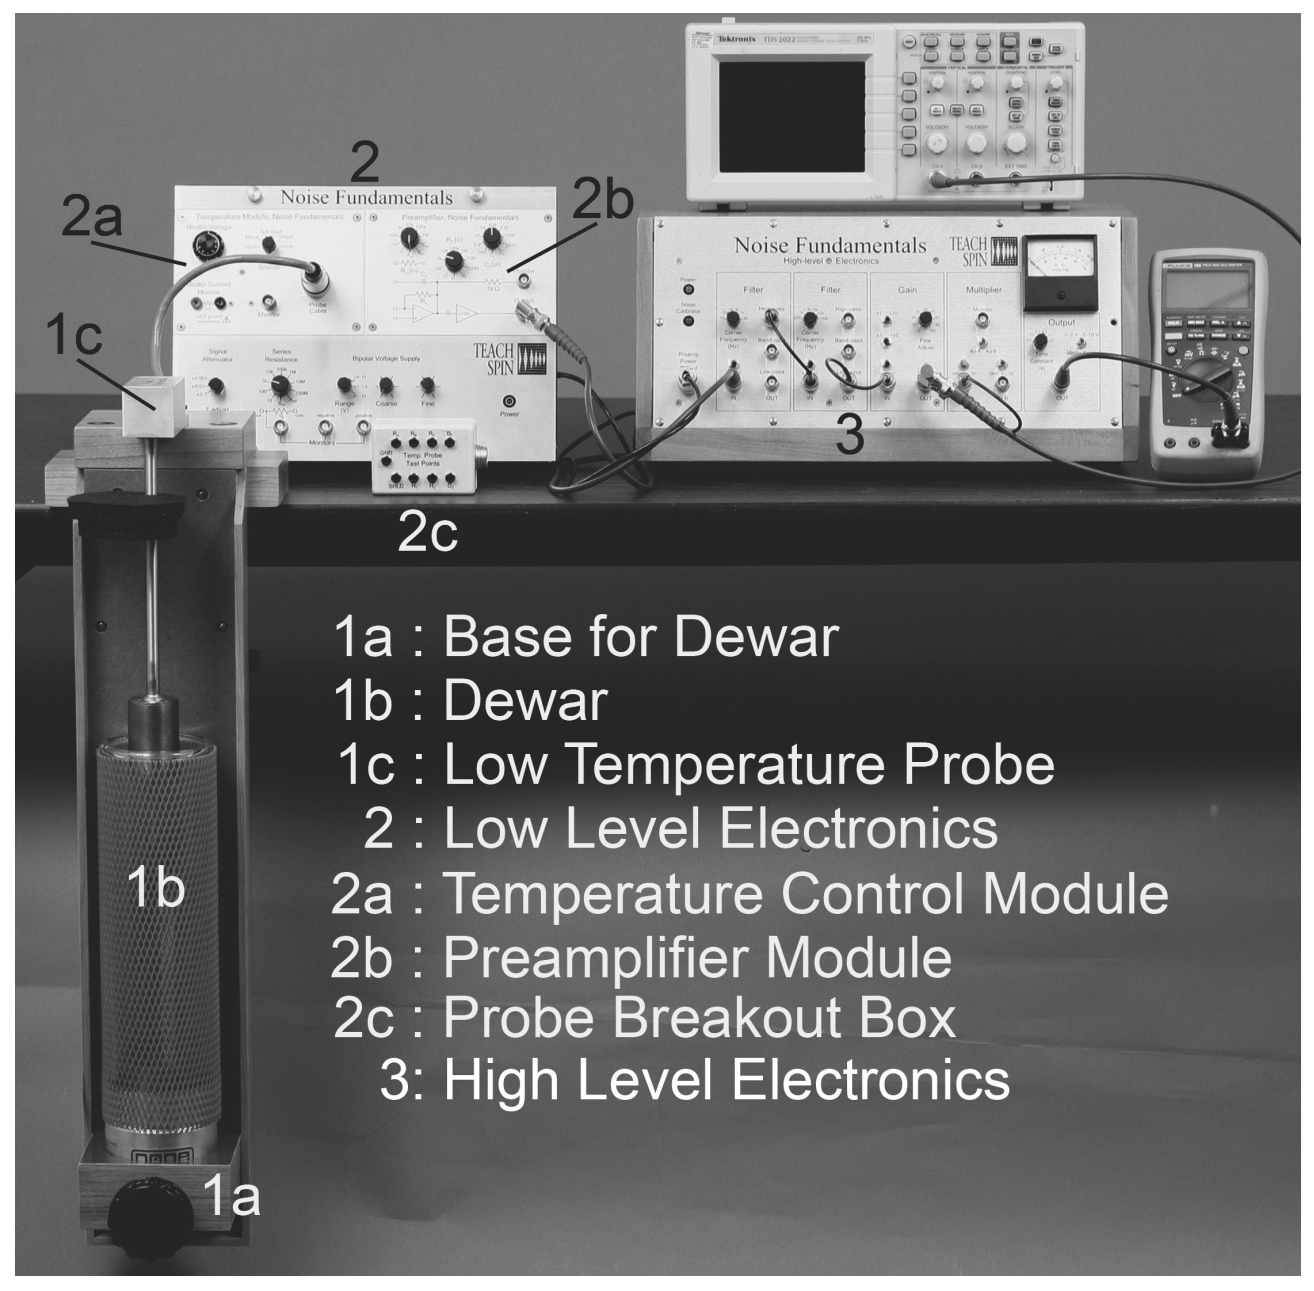
\includegraphics[width=0.5\textwidth]{Apparatus.PNG}
		\caption{Equipment diagram with labels for measuring Johnson and shot noise.}
		\label{apparatus}
	\end{wrapfigure}

	The equipment for this lab are provided in \cref{apparatus} for reference. The equipment labeled under ``2'' is the \emph{Low Level Electronics} (LLE) box. This is what provides the noise signal, Johnson or shot, and an initial amplification. The equipment under ``3'' is the \emph{High Level Electronics} (HHE) box, and allows for the signal to be filtered, further amplified, and squared before being read out to an oscilloscope or multimeter. The equipment under ``1'' is used for measuring the temperature dependence of Johnson noise. To obtain a wide temperature range, we use liquid nitrogen to cool the temperature probe. 
		
	\subsection{Measuring Johnson Noise}
	We measure the power spectral density of Johnson noise to verify Nyquist's theorem \cref{nyquistEqn} in two ways, by measuring the resistance and temperature dependence. To obtain the resistance dependence, we vary the source resistance $R_{in}$ and record the time-averaged square of the signal after being sent through the HLE box. For these measurements, the corresponding high and low pass cutoffs are $3$ kHz and $3.3$ kHz. We adjusted the gain on the HLE to 300 to see the signal clearly.
	
	To measure the temperature dependence, we submerge the temperature probe inside liquid nitrogen and adjust the temperature with the temperature control module. For these measurements, there are only three resistors inside the probe, corresponding to $R_A = 10 \text{ } \Omega$, $R_B = 10 \text{ k}\Omega$, and $R_C = 100 \text{ k}\Omega$. The data measured is presented in \cref{temp10,temp10k,temp100k} and visualized in \cref{tempGraphs}.
	
	\subsection{Measuring Shot Noise}
	We To measure the power spectral density of shot noise, we configure the LLE and HLE boxes similar to the configuration for Johnson noise. We fix the following values: $R_f = 10 \ \text{k}\Omega$ and adjust the photodiode current to $I_{\text{dc}} = 10 \ \mu \text{A}$. We begin by varying the low pass frequency and record the power spectrum as a function of bandwidth. We then fix the low pass frequency to $f_{\text{LP}} = 10 \ \text{kHz}$ and vary the photodiode current $I_{\text{dc}}$ up to $100 \ \mu \text{A}$
	
	\subsection{Corrections}
	Before proceeding with measurements, it is important to understand some corrective factors. The signal of interest is noise, Johnson or shot, but each device also contributes identical noise to the signal. Not accounting for these additions results in measurements being artificially inflated.
	
	For Johnson noise, we can model a real amplifier as an ideal amplifier with some background noise voltage $V_b$ added to its source. The measured value at the ``\texttt{out}'' terminal, $V_\text{out}$, is related to the Johnson noise, $\langle V_J \rangle$, by:
	\begin{equation}
		V_{\text{out}} = \left( \frac{(G_1 G_2)^2}{10 \ \text{V}} \right) \left( \langle V_J^2 \rangle + \langle V_b^2 \rangle \right)
	\end{equation} 
	where the factors $G_1$ and $G_2$ are the gains of the LLE and HLE.
	
	To obtain a value for the background noise voltage, we minimize the Johnson noise from the feedback resistor $R_f$ relative to the background. Setting $R_{\text{in}} = 1 \ \Omega$ allows for a direct measurement of the background noise voltage $V_{b}$.
	
	When measuring the temperature dependence we must account for the additional cable length between the temperature probe and the LLE box. This cable is a shielded coax cable which protects against external feedback, but also introduces a significant amount of capacitance between the signal lead and ground. This additional capacitance reduces the effective bandwidth of the signal. This can be seen by, at room temperature, measuring the output voltage from the resistors in the probe and inside the LLE box. The output voltage from the resistors in the probe should be smaller than from the resistors in the LLE box. To correct for this effect, we adjust the high pass filter to $3$ kHz and low pass to $3.3$ kHz, which minimizes this discrepancy between output voltages.
	
	Similar to Johnson noise, the instrumentation contributes a small amount of shot noise, $V_b$, to the signal and must be accounted for. The measured voltage from the ``\texttt{out}'' terminal on the HLE box is related to shot noise by:
	\begin{equation}
		V_{\text{out}} = \left( \frac{(100G_2)^2}{10 \ V} \right) \left( R_f^2\langle I^2_{\text{shot}} \rangle + \langle V_b \rangle \right)
	\end{equation}
	
	It is possible to directly measure the noise contribution from the instrumentation by turning the photodiode current,$I_{dc}$ and thus the shot current $I_{\text{shot}}$, to zero.
	
	\section{Results and Analysis}

	\subsection{Johnson Noise}
	\subsubsection*{Resistance Dependence}
	Plotting measured values, see \cref{johnsonRTable}, for the power spectral density against resistance, we obtain \cref{powerR}. The x-axis is plotted on a logarithmic scale because the resistance values span five orders of magnitude. The best-fit line is a linear fit obeying $S = 1.18\times 10^{-20}R$.
	
	\begin{figure}[H]
		\centering
		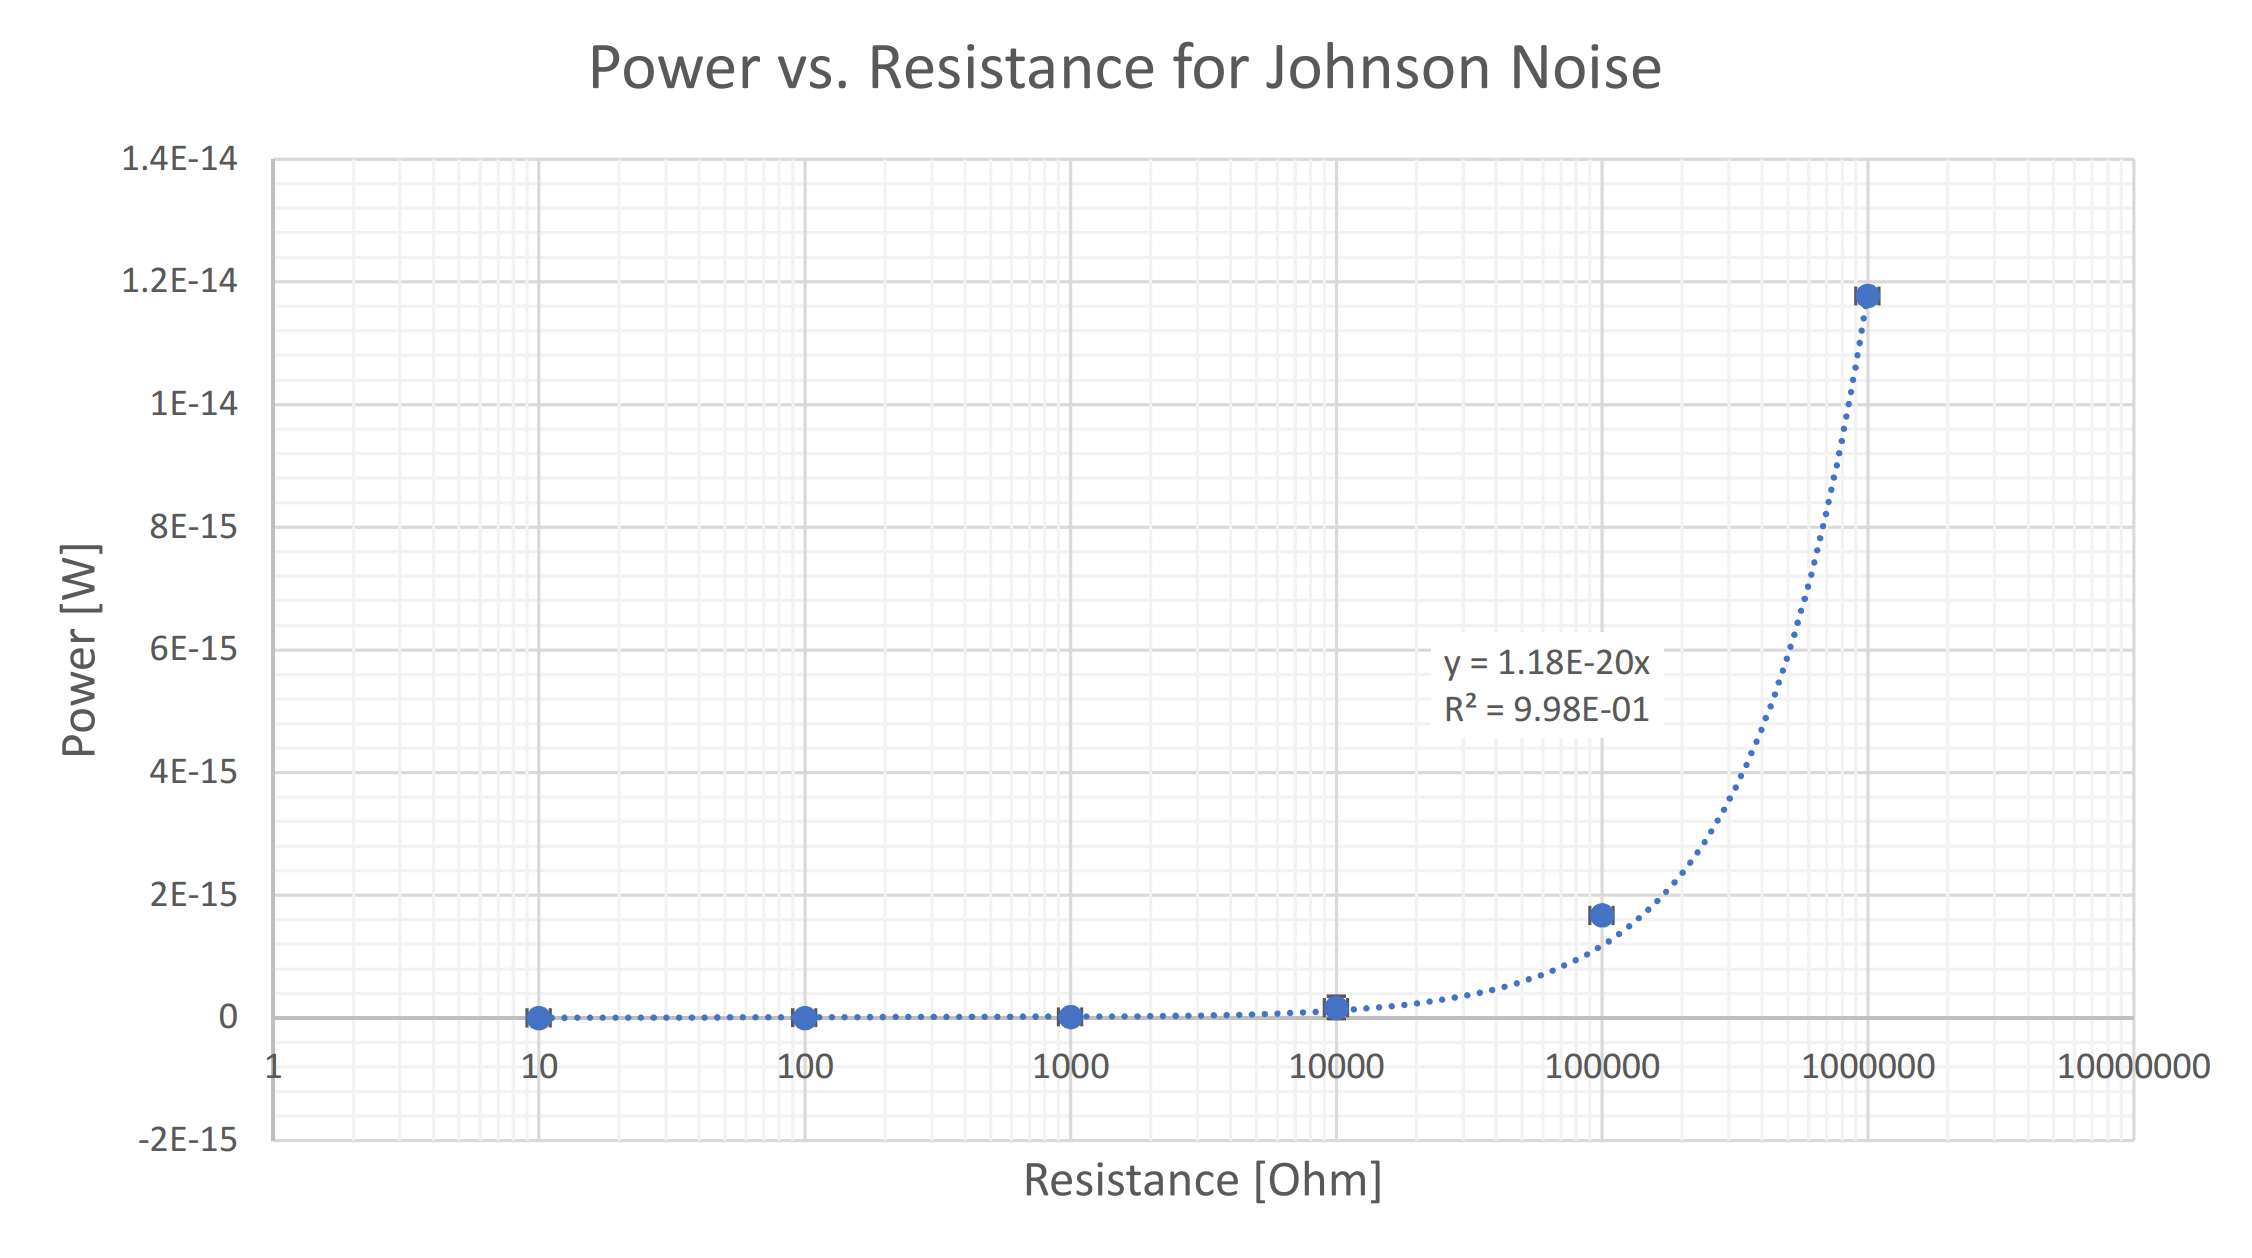
\includegraphics[width=0.8\textwidth]{powerR.png}
		\caption{Graph of power spectral density versus resistance for Johnson noise, see \cref{johnsonRTable}}
		\label{powerR}
	\end{figure}

	From Nyquist's Theorem, \cref{nyquistEqn}, we can equate the slope to $4k_BT$ and extract Boltzmann's constant:
	\begin{equation}
		k_B = 1.00 \times 10^{-23} \pm 2.15\times 10^{-23}
	\end{equation}
	
	
	
	\subsubsection*{Temperature Dependence}
	To obtain date for the temperature dependence, we use the three resistors inside the temperature probe, which are $10 \ \Omega$, $10 \ \text{k}\Omega$ and $100 \ \text{k}\Omega$ respectively. We find that the $10 \ \text{k}\Omega$ and $100 \ \text{k}\Omega$ resistors provide reliable data, but the fluctuations in the $10 \ \Omega$ resistor are too small to measure with the provided multimeters. In \cref{tempGraphs}, we plot the data provided in the Appendix in \cref{temp10,temp10k,temp100k}.
	
	\begin{figure}[H]
		\centering
		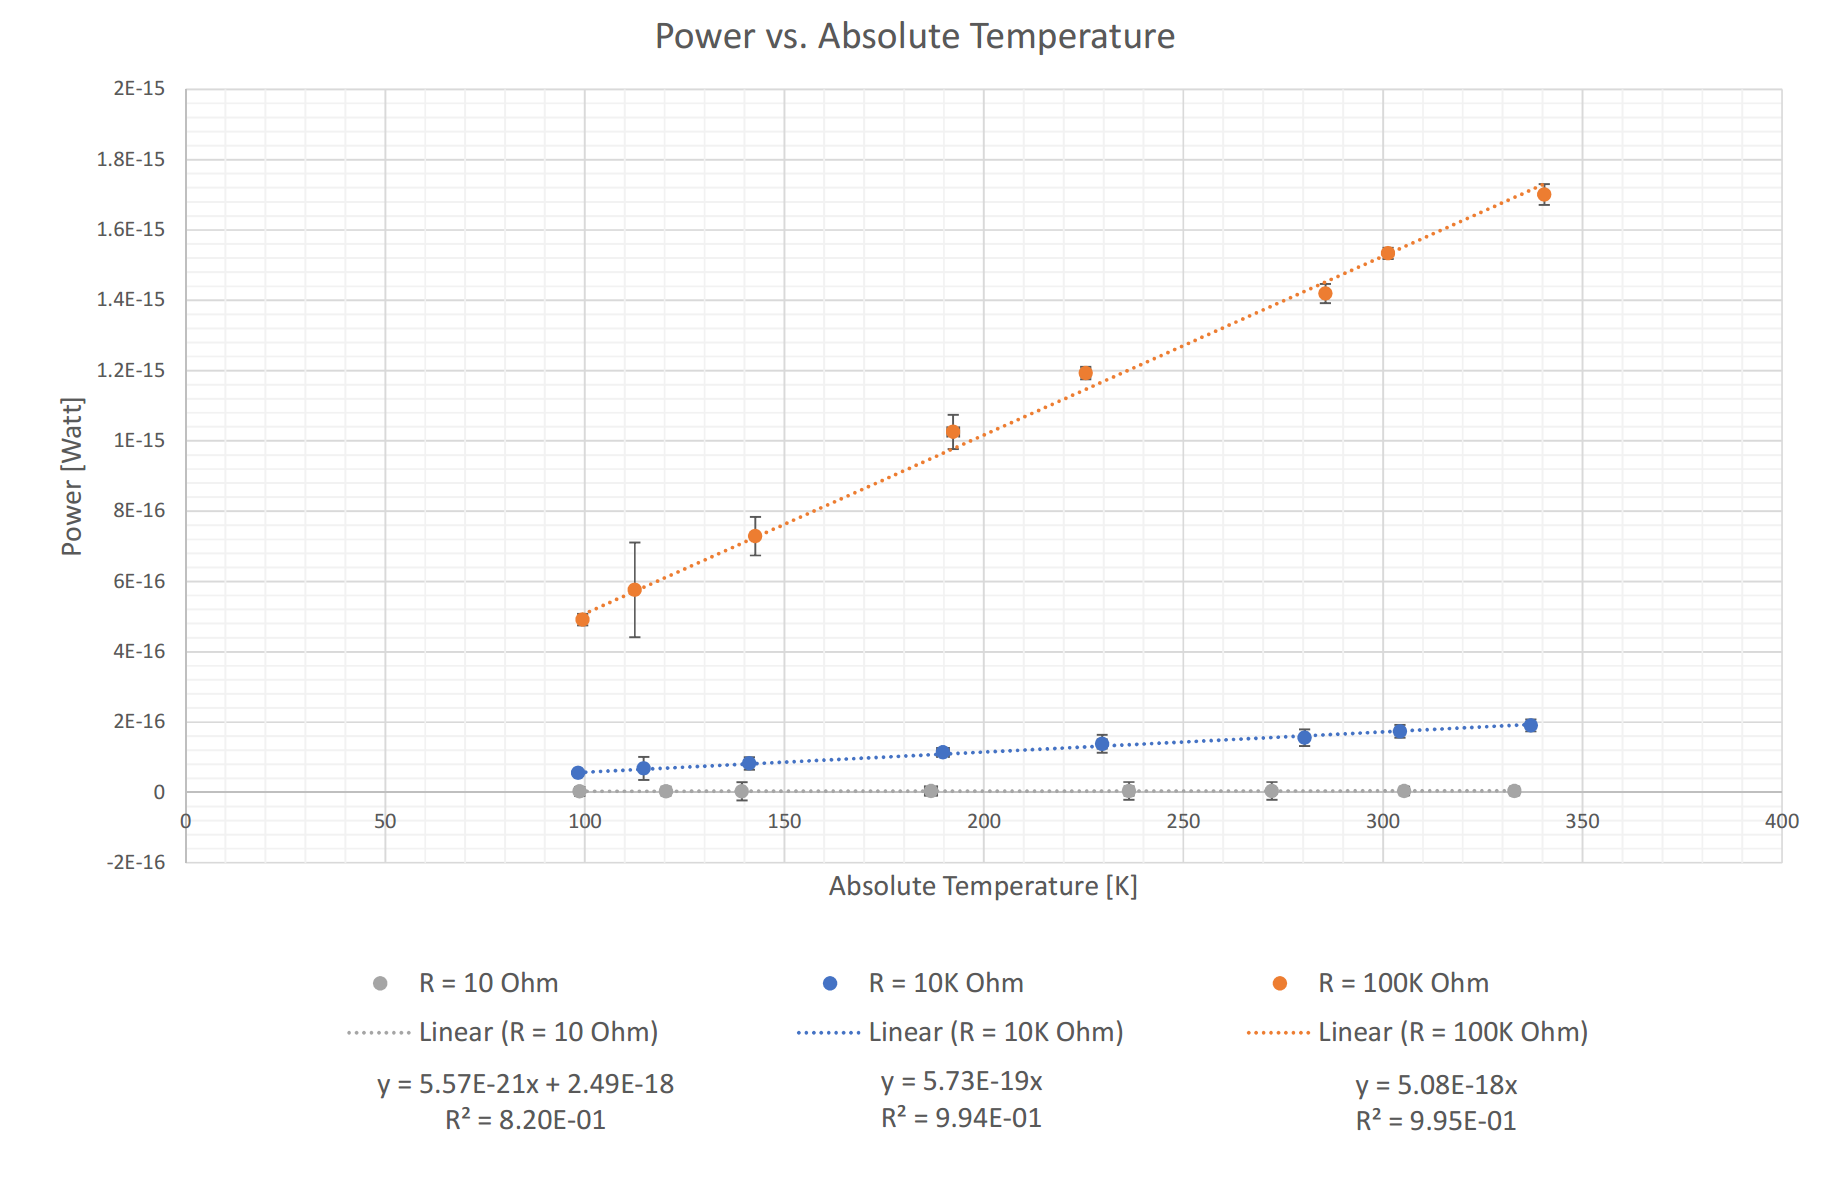
\includegraphics[width=0.8\textwidth]{TempGraph.PNG}
		\caption{Graph of Power spectral density versus absolute temperature for $10$ $\Omega$, $10$ k$\Omega$ and $100$ k$\Omega$ resistors.}
		\label{tempGraphs}
	\end{figure}

	In choosing the fit-lines, we require the physical constraint that at zero temperature, there is no power emitted from the resistor, which fixes the vertical intercept to be zero. For the $10$ k$\Omega$ and $100$ k$\Omega$ resistors, this condition yielded $R^2$ values very close to 1, indicating that the data follows a linear fit.
	
	\begin{wraptable}{l}{0.45\textwidth}
		\begin{tabular}{l c}
			\toprule
			\textbf{Resistor} & $\mathbf{k_B}$ \\ \toprule
			$10 \ \Omega$ & $1.39\times 10^{-22} \pm 3.75\times 10^{-24}$ \\
			$10 \ k\Omega$ & $1.43\times 10^{-23} \pm 1.44\times10^{-25}$\\
			$100 \ k\Omega$ & $1.27 \times 10^{-23} \pm 1.30\times10^{-25} $ \\ 
			\bottomrule			
		\end{tabular}
		\caption{Table summarizing the measured Boltzmann constants from temperature data}
		\label{BoltzmannTable}
	\end{wraptable}
	
	However, imposing this same condition on the $10$ $\Omega$ resistor resulted in a negative $R^2$ value. We attribute this to two reasons. First, referring to \cref{temp10}, the power measurements fluctuate very little, which indicates that our multimeters are not sensitive enough to measure significant changes in the signal. Secondly, because there are only 4 unique power measurements, Microsoft Excel is unable to create a best fit line which simultaneously fits the data and passes through the origin. To alleviate this problem, we lift the physical constraint, that at zero absolute temperature we expect zero noise, and obtain the presented $R^2$ value. 
	
	Equating the slopes of the best-fit lines to the corresponding factor in Nyquist's equation, \cref{nyquistEqn}, we obtain the values for Boltzmann's constant listed in \cref{BoltzmannTable}. Averaging these values and errors, yields:
	\begin{equation}
		k_B = 5.54 \times 10^{-23} \pm 5.56 \times 10 ^{-23}		
	\end{equation}

	
	\subsection{Shot Noise}
	We plot the power spectral density of shot noise against bandwidth, \cref{shotBandwidth} and photodiode current, \cref{shotCurrent}. We can see that in both cases, the data obeys a linear relation predicted by Schottky's theorem, \cref{schottkyEqn}. Data tables for both graphs are provided in the appendix in \cref{shotBandwidthTable,shotCurrentTable}.

	\begin{figure}[H]
		\centering
		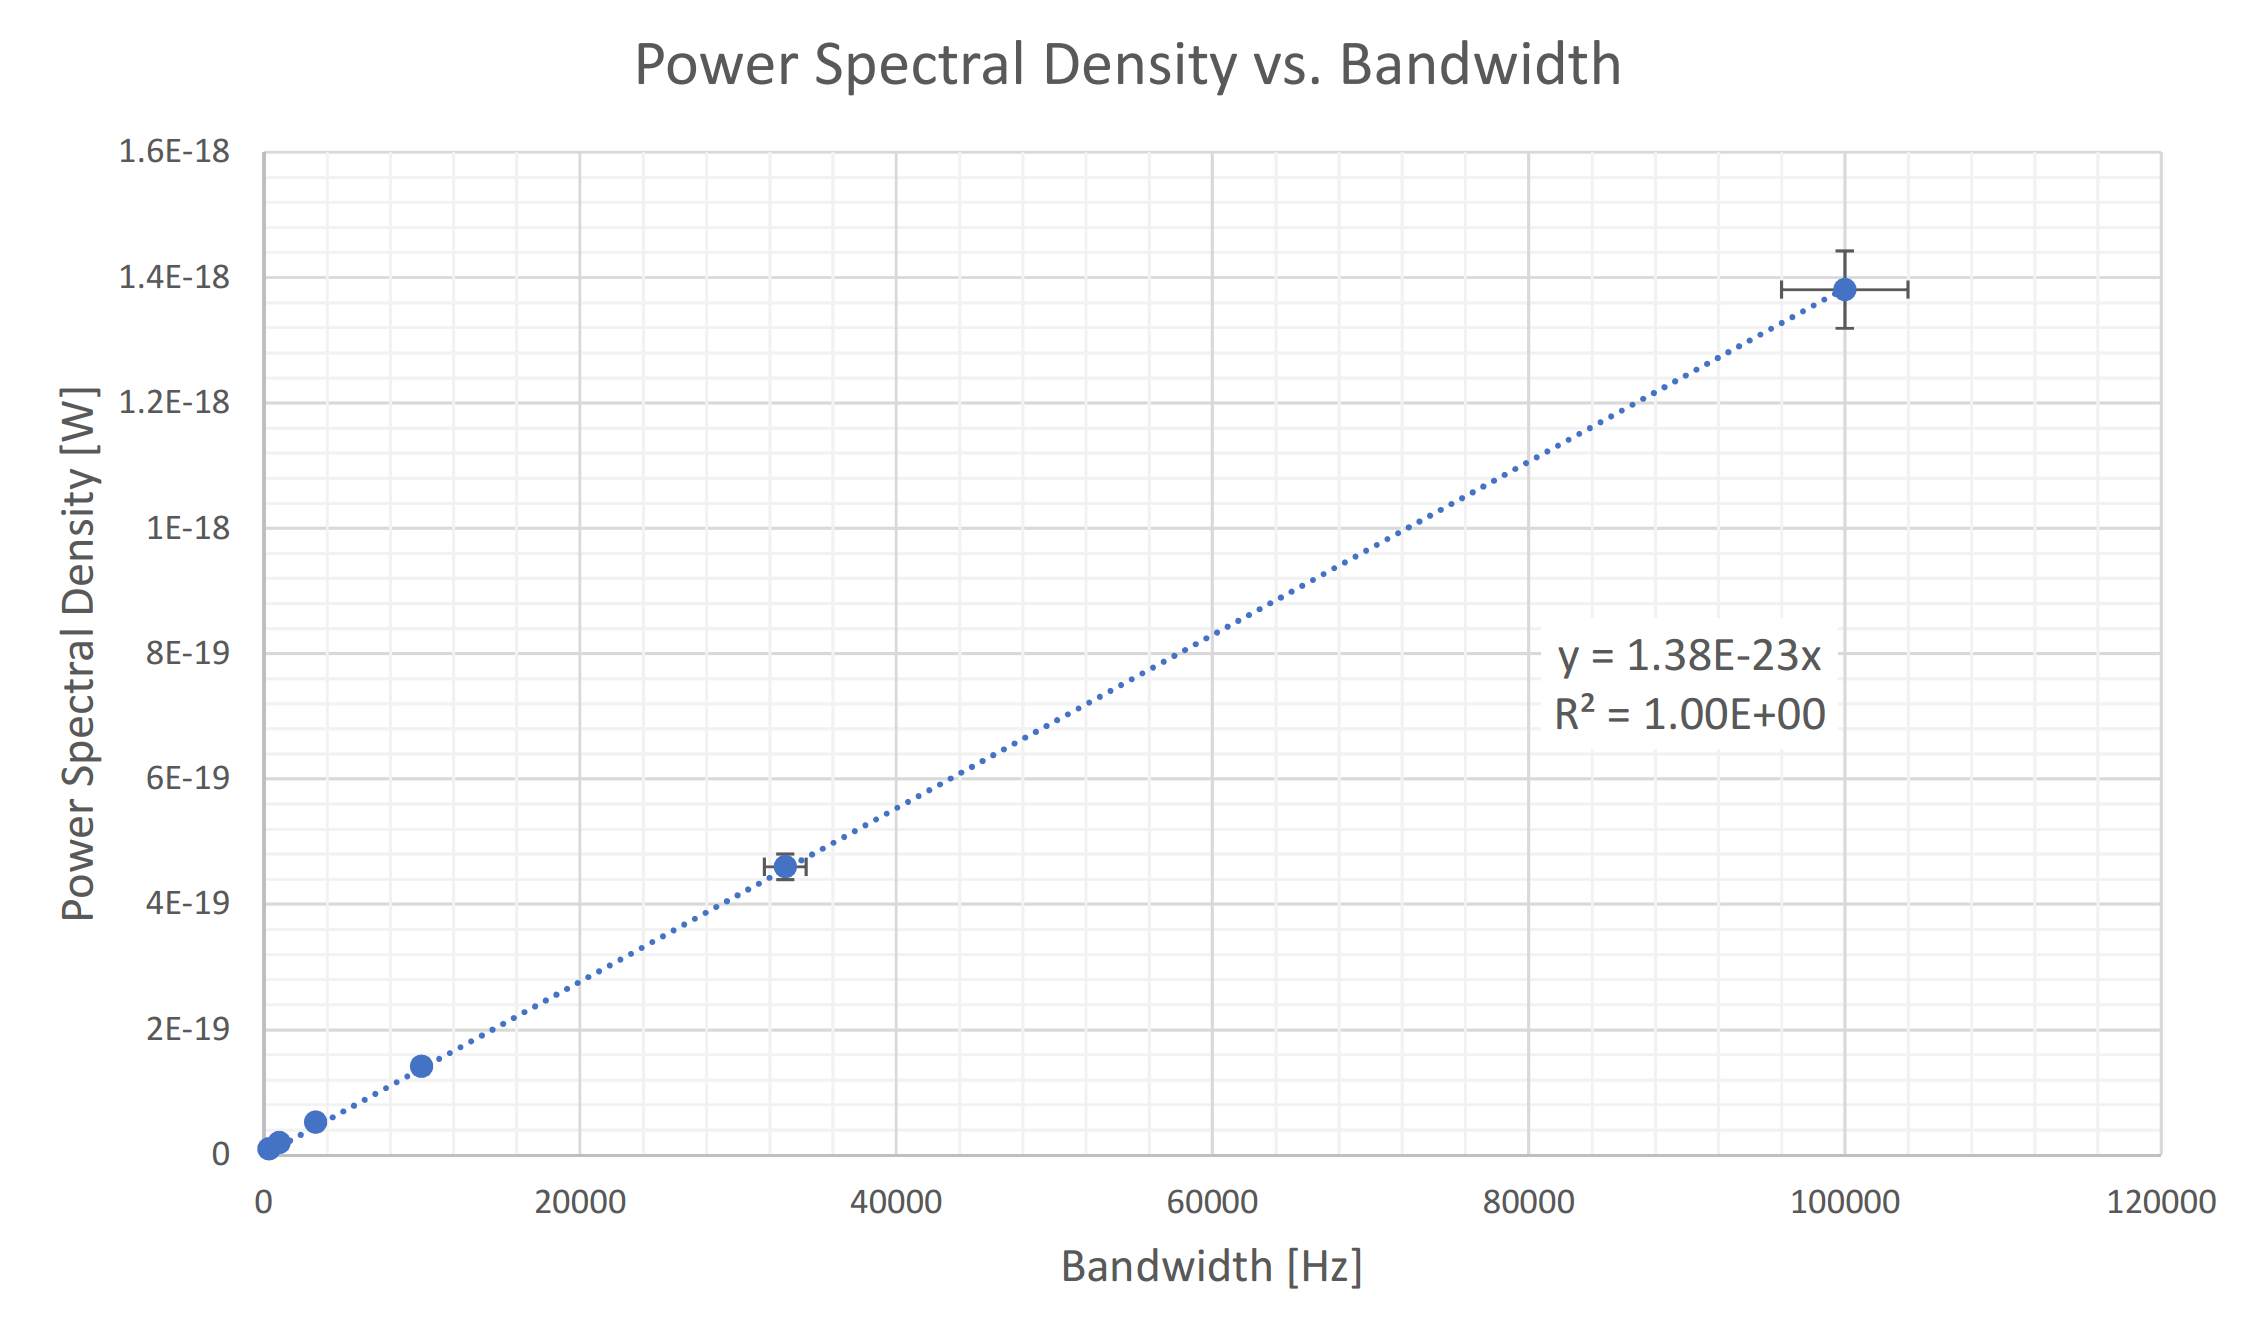
\includegraphics[width=0.6\textwidth]{ShotBandwidth.PNG}
		\caption{Power spectral density versus bandwidth for shot noise}
		\label{shotBandwidth}
	\end{figure}
	
	\begin{figure}[H]
		\centering
		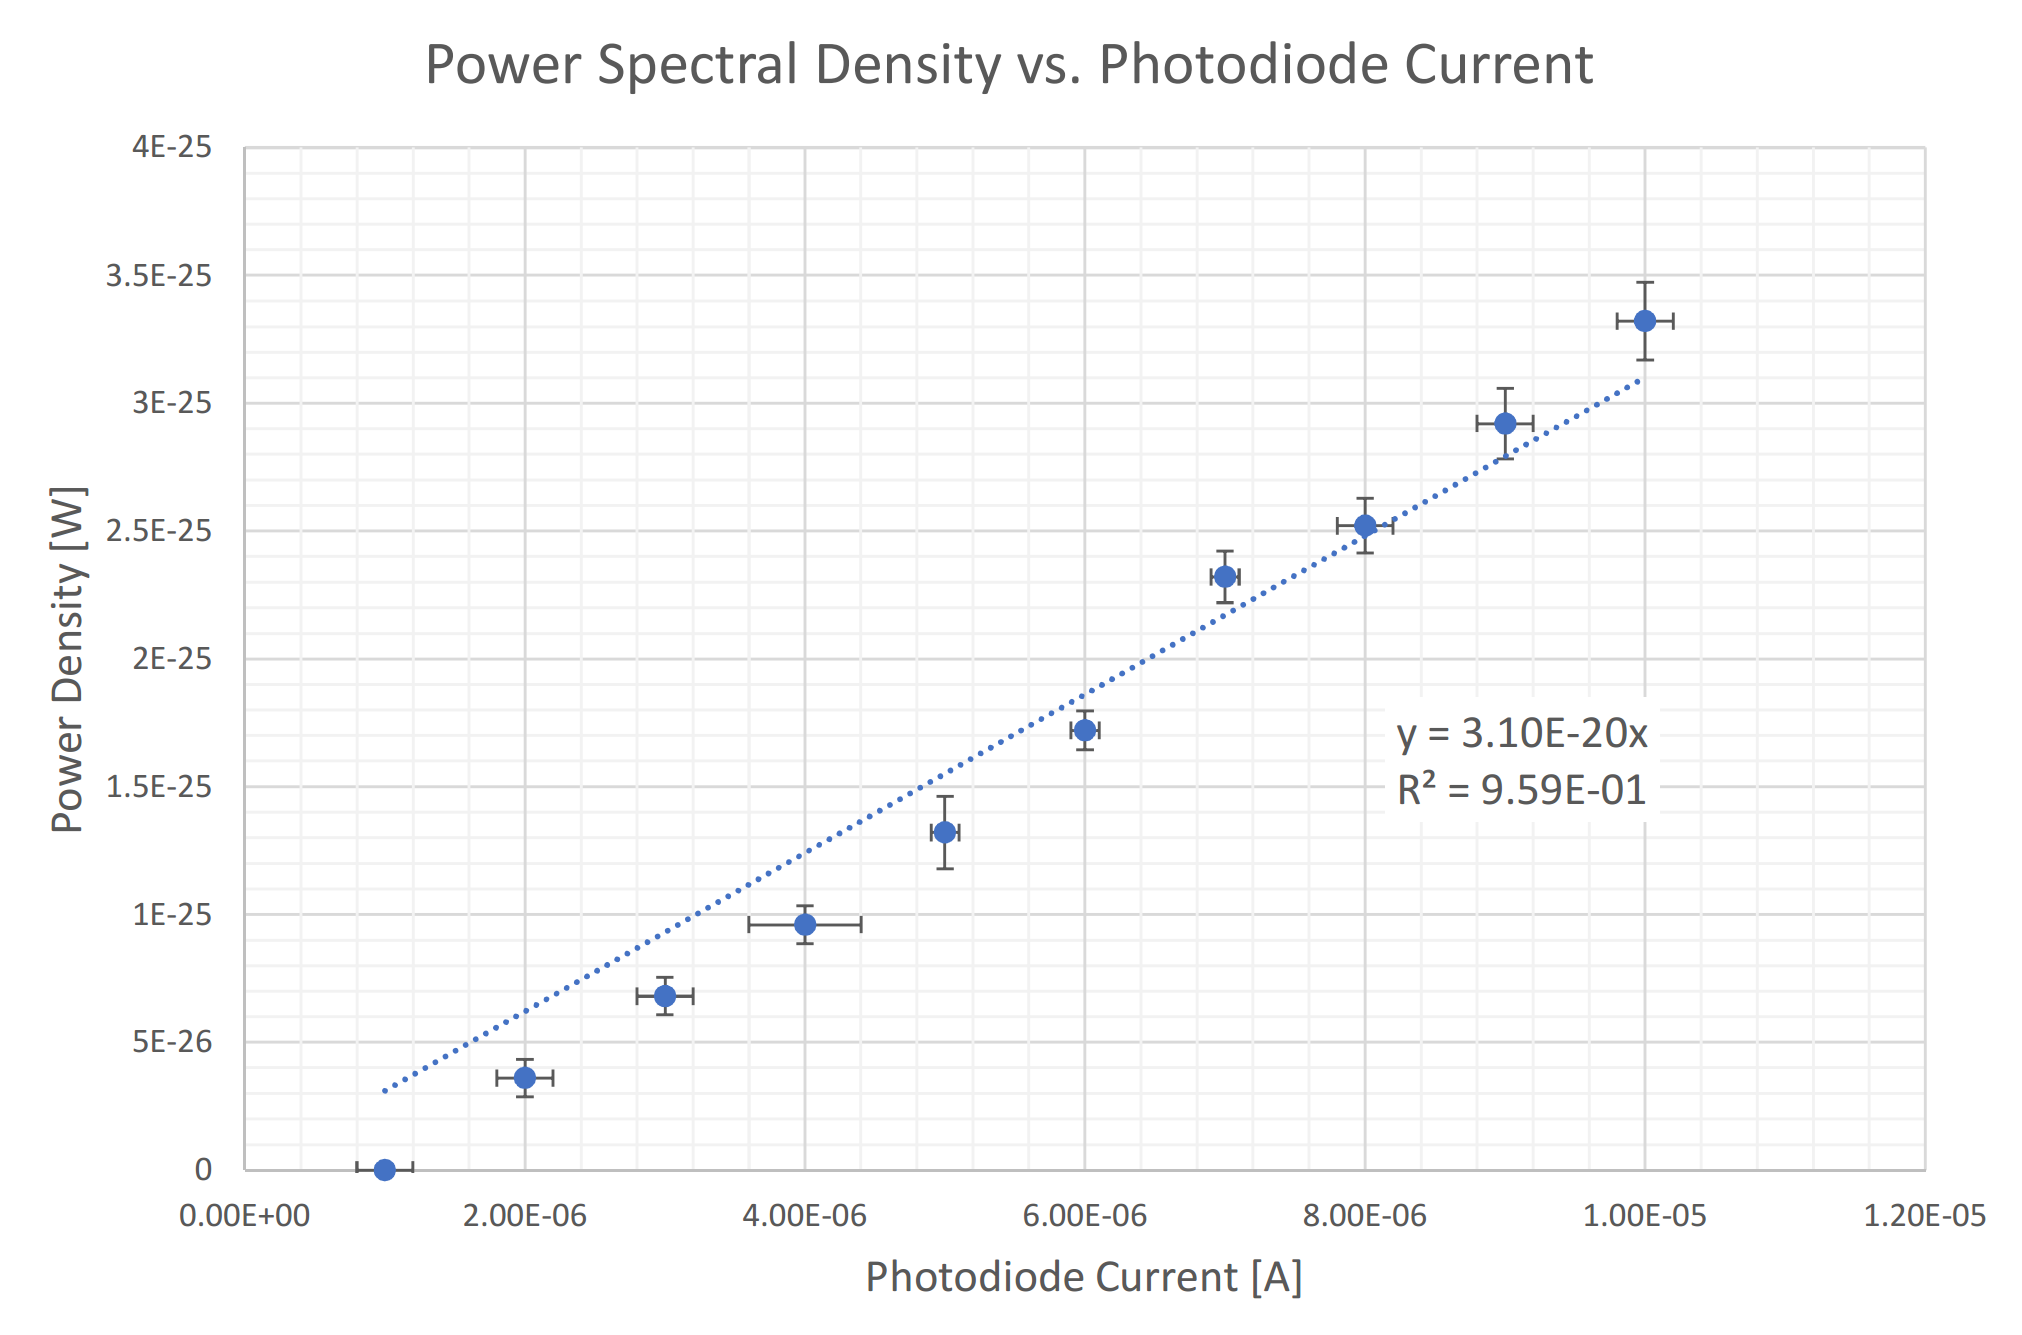
\includegraphics[width=0.6\textwidth]{ShotCurrent.PNG}
		\caption{Power spectral density versus photodiode current for shot noise}
		\label{shotCurrent}
	\end{figure}
	
	In \cref{shotBandwidth}, we note that the power spectrum is not white. If the noise was white, the power spectrum would be flat. However for shot noise,  larger bandwidths allow more power to be transmitted which is why the slope is non-zero.
	
	Further, since both graphs are linear, we can equate the slopes to the corresponding factor in \cref{schottkyEqn} and extract the charge of the electron. \cref{bandwidthE,currentE} show the charge of the electron from the bandwidth and current graphs respectively.
	\begin{equation}
		e = 6.21 \times 10^{-19} \pm 3.73 \times 10^{-20}
		\label{bandwidthE}
	\end{equation}

	\begin{equation}
		e= 1.52 \times 10^{-20} \pm 1.64 \times 10^{-21}
		\label{currentE}
	\end{equation}
	
	\section{Conclusion}
	
	\subsubsection*{Accomplishments}
	In this experiment we verify that Nyquist's theorem successfully predicts how Johnson noise depends on resistance and temperature. From this prediction, we are able to measure Boltzmann's constant to be \red{Kb}. Additionally, we also verify that Schottky's theorem successfully predicts how shot noise depends on bandwidth and photodiode current. From Schottky's theorem, we are able to measure the fundamental electric charge to be \red{e}.
	
	\subsubsection*{Improvements and Future Experiments}
	While measuring shot noise, we noticed that the voltage measurements are extremely sensitive to vibrations and especially talking. We did our best to minimize our talking, but we could not eliminate the ambient sound in the room. It would be interesting to repeat this experiment in an anechoic chamber to further reduce the literal background noise. 
	
	
	\pagebreak
	\section*{Appendix}

\subsection*{Resistor Dependence}

\begin{table}[H]
	\centering
	\begin{tabular}{l l c c} \toprule
		\textbf{R} $\mathbf{[\Omega]}$ & $\mathbf{\delta R \ [\Omega]}$ & \textbf{S [W]}   & $\mathbf{\delta S \ [W]}$  \\ \toprule
		10      & 0.04 & 6.43E-17 & 1.34E-17 \\
		100     & 0.4  & 6.72E-17 & 1.28E-17 \\
		1000    & 4    & 8.08E-17 & 1.07E-17 \\
		10000   & 40   & 2.33E-16 & 1.85E-16 \\
		100000  & 400  & 1.74E-15 & 2.29E-17 \\
		1000000 & 4000 & 1.18E-14 & 1.19E-16 \\
		\bottomrule  
	\end{tabular}
	\caption{Table of measured values for resistance and power for Johnson noise}
	\label{johnsonRTable}
\end{table}

\subsection*{Temperature Dependence Data}
The following graph shows the conversion between voltage and absolute temperature. The data is provided in the laboratory manual.

\begin{figure}[H]
	\centering
	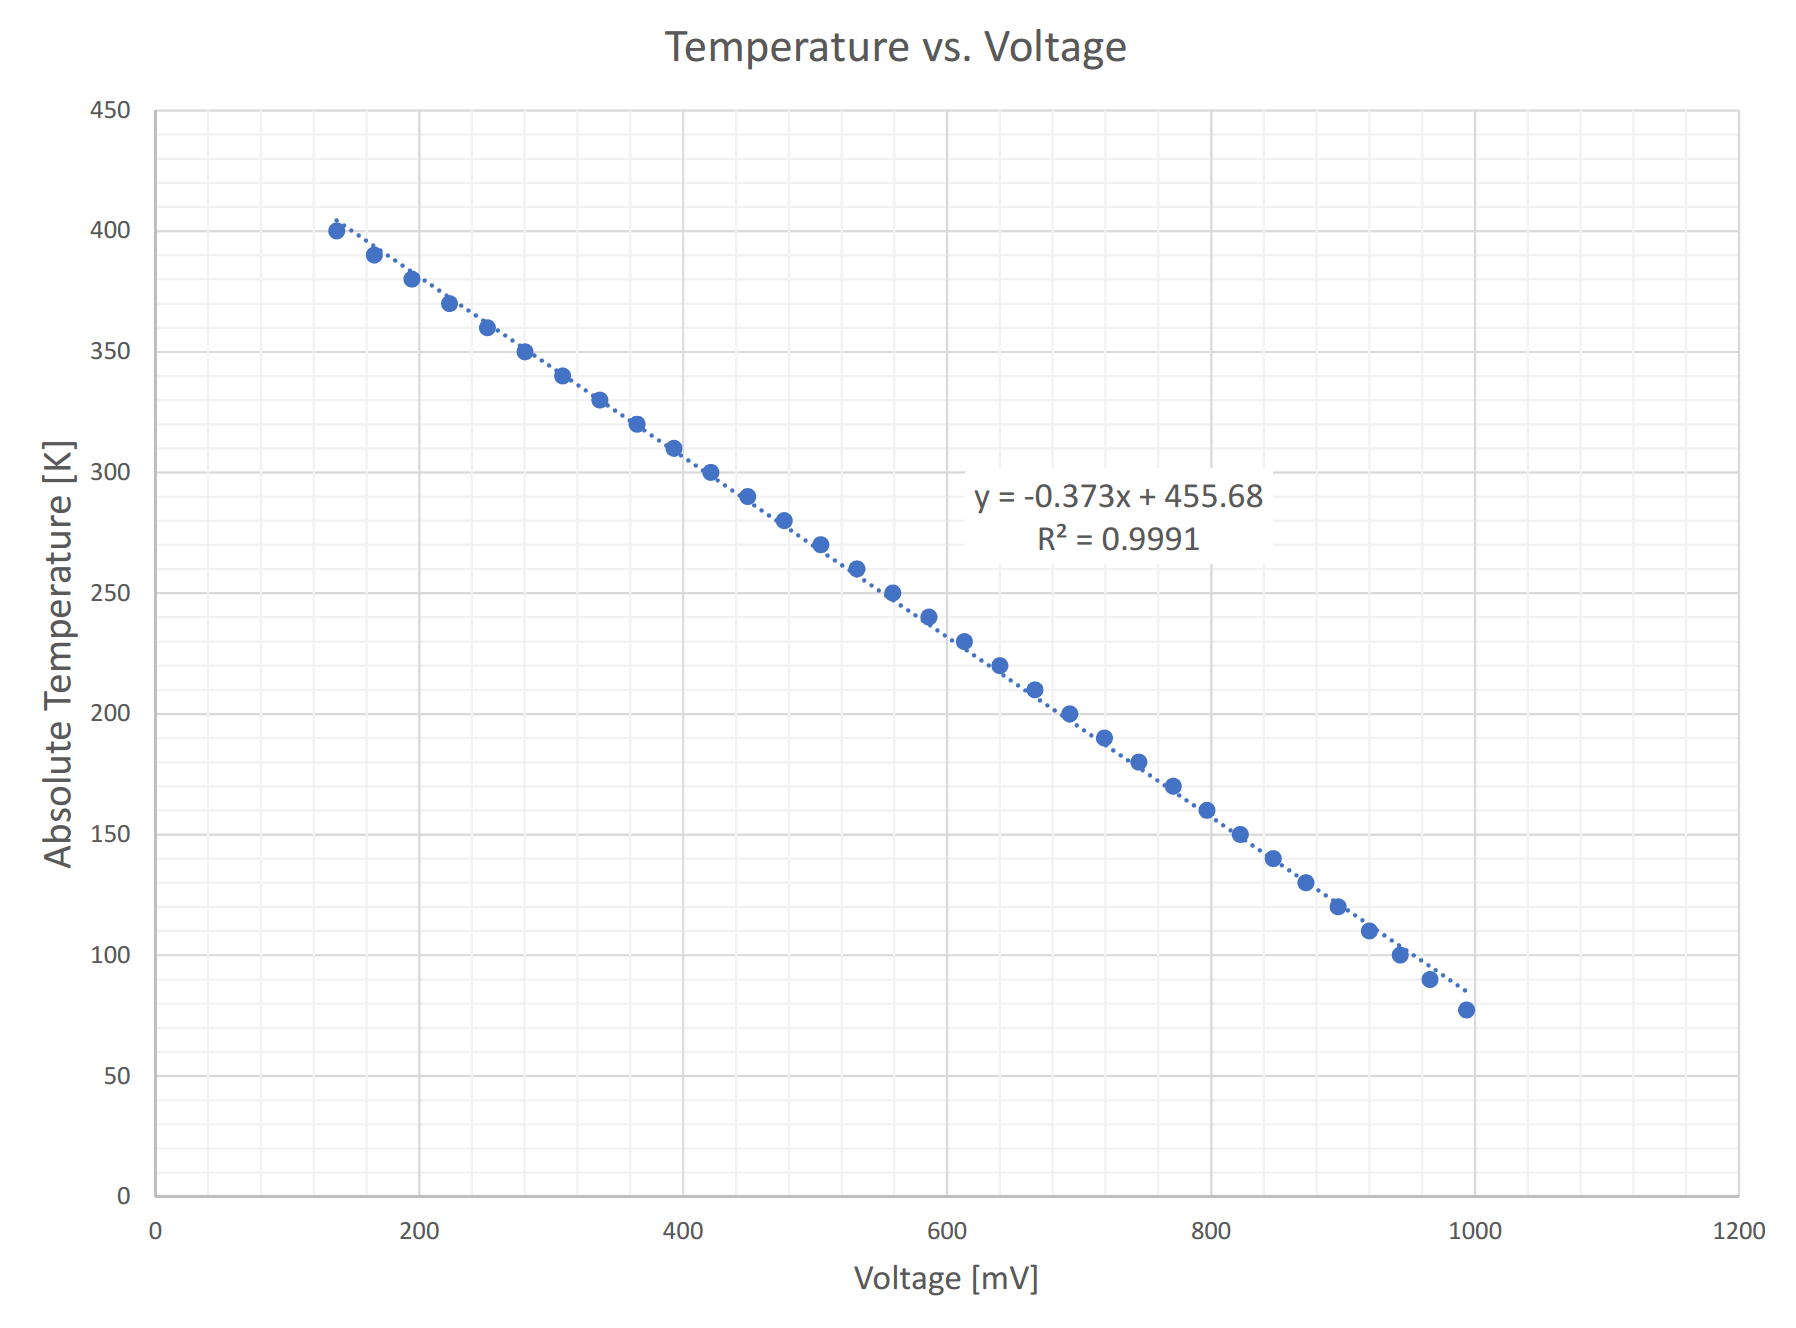
\includegraphics[width=0.7\textwidth]{TVConversion.PNG}
	\caption{Conversion between voltage and absolute temperature for a photodiode at constant $10 \ \mu A$ current.}
	\label{tvgraph}
\end{figure}


\begin{table}[H]
	\centering
	\begin{tabular}{c c c c} \toprule
		\textbf{Temp [K]} & $\mathbf{\delta}$\textbf{T [K]} & \textbf{Power [W]} & $\mathbf{\delta}$\textbf{S} \\ \toprule
		98.7 & 0.746 & 2.94E-18 & 1.29E-17 \\
		120  & 0.746 & 3.23E-18 & 1.28E-17 \\
		139  & 0.746 & 2.94E-18 & 2.58E-17 \\
		187  & 1.49  & 3.82E-18 & 1.27E-17 \\
		236  & 1.12  & 4.11E-18 & 2.53E-17 \\
		272  & 0.746 & 4.11E-18 & 2.53E-17 \\
		305  & 0.746 & 4.11E-18 & 1.27E-17 \\
		333  & 0.746 & 4.11E-18 & 1.27E-17 \\
		\bottomrule  
	\end{tabular}
	\caption{Temperature Dependence for R = 10 $\Omega$}
	\label{temp10}
\end{table}



\begin{table}[H]
	\centering
	\begin{tabular}{c c c c} \toprule
		\textbf{Temp [K]} & $\mathbf{\delta}$\textbf{T [K]} & \textbf{Power [W]} & $\mathbf{\delta}$\textbf{S} \\ \toprule
		98.3 & 0.746 & 5.52E-17 & 7.25E-18 \\
		115  & 0.746 & 6.78E-17 & 3.27E-17 \\
		141  & 0.746 & 8.22E-17 & 1.77E-17 \\
		190  & 1.49  & 1.14E-16 & 9.77E-18 \\
		230  & 1.12  & 1.38E-16 & 2.56E-17 \\
		280  & 0.746 & 1.56E-16 & 2.36E-17 \\
		304  & 0.746 & 1.74E-16 & 1.82E-17 \\
		337  & 0.746 & 1.90E-16 & 1.71E-17 \\
		\bottomrule
	\end{tabular}
\caption{Temperature Dependence for R = 10 k$\Omega$}
\label{temp10k}
\end{table}



\begin{table}[H]
	\centering
	\begin{tabular}{cccc} \toprule
		\textbf{Temp [K]} & $\mathbf{\delta}$\textbf{T [K]} & \textbf{Power [W]} & $\mathbf{\delta}$\textbf{S} \\ \toprule
		99.5 & 0.746 & 4.91E-16 & 1.63E-17 \\
		113  & 0.746 & 5.76E-16 & 1.35E-16 \\
		143  & 0.746 & 7.29E-16 & 5.49E-17 \\
		192  & 1.49  & 1.03E-15 & 4.86E-17 \\
		226  & 1.12  & 1.19E-15 & 1.82E-17 \\
		286  & 0.746 & 1.42E-15 & 2.72E-17 \\
		301  & 0.746 & 1.53E-15 & 1.63E-17 \\
		340  & 0.746 & 1.70E-15 & 2.98E-17 \\
		\bottomrule
	\end{tabular}
	\caption{Temperature Dependence for R = 100 k$\Omega$}
	\label{temp100k}
\end{table}


\subsection*{Shot Noise}

\begin{table}[H]
	\centering
	\begin{tabular}{cccc} \toprule
		$\mathbf{\Delta f}$ & $\mathbf{\delta (\Delta f)}$ & $\mathbf{\langle s \rangle}$ & $\mathbf{\delta \langle s \rangle}$ \\ \toprule
		314   & 12.56   & 9.68E-21 & 4.33E-22 \\
		984   & 39.36   & 1.97E-20 & 8.80E-22 \\
		3284  & 131.36  & 5.23E-20 & 2.34E-21 \\
		9984  & 399.36  & 1.42E-19 & 6.33E-21 \\
		32984 & 1319.36 & 4.60E-19 & 2.06E-20 \\
		99984 & 3999.36 & 1.38E-18 & 6.18E-20 \\
		\bottomrule
	\end{tabular}
	\caption{Data collected for power spectral density versus bandwidth for shot noise}
	\label{shotBandwidthTable}
\end{table}


\begin{table}[H]
	\centering
	\begin{tabular}{cccc} \toprule
		$\mathbf{I_{dc}}$ & $\mathbf{\delta (I_{dc})}$ & $\mathbf{\langle s \rangle}$ & $\mathbf{\delta \langle s \rangle}$ \\ \toprule
		1.00E-06 & 2.00E-07 & 3.21E-26 & 6.66E-27 \\
		2.00E-06 & 2.00E-07 & 9.62E-26 & 1.10E-26 \\
		3.00E-06 & 2.00E-07 & 1.16E-25 & 1.02E-26 \\
		4.00E-06 & 4.00E-07 & 1.48E-25 & 1.70E-26 \\
		5.00E-06 & 1.00E-07 & 1.76E-25 & 1.06E-26 \\
		6.00E-06 & 1.00E-07 & 2.00E-25 & 1.18E-26 \\
		7.00E-06 & 1.00E-07 & 2.44E-25 & 1.43E-26 \\
		8.00E-06 & 2.00E-07 & 2.80E-25 & 1.73E-26 \\
		9.00E-06 & 2.00E-07 & 3.17E-25 & 1.92E-26 \\
		1.00E-05 & 2.00E-07 & 3.65E-25 & 2.19E-26 \\
		\bottomrule
	\end{tabular}
	\caption{Data collected for power spectral density versus photodiode current for shot noise}
	\label{shotCurrentTable}
\end{table}
%
%	
%	\pagebreak
%	\bibliographystyle{utphys}
%	\bibliography{references}
%	\nocite{*}

	
\end{document}
